\documentclass[12pt,pdf,hyperref={unicode}]{beamer}


%\documentclass[10pt]{beamer}

\usetheme[progressbar=frametitle]{metropolis}

\usepackage{booktabs}
\usepackage[scale=2]{ccicons}

\usepackage{pgfplots}
\usepgfplotslibrary{dateplot}

\usepackage{xspace}
\newcommand{\themename}{\textbf{\textsc{metropolis}}\xspace}


%\usepackage{lmodern}

% подключаем кириллицу 
\usepackage[T2A]{fontenc}
\usepackage[utf8]{inputenc}
\usepackage{listings}
%\usepackage{graphicx}
\usepackage{hyperref}

% отключить клавиши навигации
\setbeamertemplate{navigation symbols}{}

% тема оформления
\usetheme{Pittsburgh}

% цветовая схема
\usecolortheme{default}

\definecolor{light-gray}{gray}{0.90}

\title{Семинар №10}   
\subtitle{ФАКИ \the\year}
\author{Бирюков В. А.} 
\date{\today}
% \logo{
\includegraphics[height=5mm]{images/logo.png}\vspace{-7pt}}

\begin{document}

\lstset{language=C}

% титульный слайд
\begin{frame}
\titlepage
\end{frame} 



\defverbatim[colored]\makeset{
\begin{lstlisting}[language=C++,basicstyle=\ttfamily,keywordstyle=\color{blue}]
void make_set(int X) {
  parent[X] = X;
}
\end{lstlisting}
}

\lstset{
  language=C,                % choose the language of the code
  basicstyle=\ttfamily,
  columns=fixed,
  fontadjust=true,
  basewidth=0.5em,
  keywordstyle=\color{blue}\bfseries,
  commentstyle=\color{gray},
  stringstyle=\ttfamily\color{yellow!40!red},
  showstringspaces=false,
  %numbers=false,                   % where to put the line-numbers
  numbersep=5pt,
  numberstyle=\tiny\color{gray},
  numberfirstline=true,
  stepnumber=1,                   % the step between two line-numbers.        
  numbersep=5pt,                  % how far the line-numbers are from the code
  backgroundcolor=\color{white!90!gray},  % choose the background color. You must add \usepackage{color}
  showstringspaces=false,         % underline spaces within strings
  captionpos=b,                   % sets the caption-position to bottom
  breaklines=true,                % sets automatic line breaking
  breakatwhitespace=true,         % sets if automatic breaks should only happen at whitespace
}
\lstset{literate=%
   *{0}{{{\color{red!20!violet}0}}}1
    {1}{{{\color{red!20!violet}1}}}1
    {2}{{{\color{red!20!violet}2}}}1
    {3}{{{\color{red!20!violet}3}}}1
    {4}{{{\color{red!20!violet}4}}}1
    {5}{{{\color{red!20!violet}5}}}1
    {6}{{{\color{red!20!violet}6}}}1
    {7}{{{\color{red!20!violet}7}}}1
    {8}{{{\color{red!20!violet}8}}}1
    {9}{{{\color{red!20!violet}9}}}1
}



\section{Форматированный ввод/вывод}

\begin{frame}[fragile]
\frametitle{Функции printf(), scanf() и sprintf(), sscanf()} 
Считывание и печать даты в формате: YYYY-MM-DD. \\
Например "2008-10-5".\\
Из стандартного входа в стандартный выход:
\begin{lstlisting}
int year, month, day;
printf("%d-%2d-%2d", 2008, 10, 5);
scanf("%d-%d-%d", &year, &month, &year);
\end{lstlisting}
Из строки в строку:
\begin{lstlisting}
char str1[20];
sprintf(str1, "%d-%2d-%2d", 2008, 10, 5);
char str2[20] = "2010-5-2";
sscanf(str2, "%d-%d-%d", &year, &month, &day);
\end{lstlisting}
\end{frame}

\begin{frame}[fragile]
\frametitle{Конвертация чисел в строку и наоборот} 
Конвертация чисел в строки с помощью sprintf():
\begin{lstlisting}
float x = 687.74564;
char str1[20];
sprintf(str1, "%f", x);
\end{lstlisting}
Конвертация строк в числа с помощью sscanf():
\begin{lstlisting}
float x;
char str2[20] = "687.74564";
sscanf(str2, "%f", &x);
\end{lstlisting}
\end{frame}




\section{Работа с файлами}

\begin{frame}[fragile]
\frametitle{Работа с файлами} 
\framesubtitle{Открываем/закрываем файл} 
\begin{lstlisting}
#include <stdio.h>

int main()
{
    FILE* fp = fopen("myfile.txt", "w");
    // ...
    fclose(fp);
}
\end{lstlisting}
\end{frame}

\begin{frame}[fragile]
\frametitle{Работа с файлами} 
\framesubtitle{Функции fprintf() и fscanf()} 
\begin{lstlisting}
#include <stdio.h>

int main()
{
    FILE* fp = fopen("myfile.txt", "r+");
        
    int year, month, day;
    fscanf(fp, "%d-%d-%d", &year, &month, &day);
    fprintf(fp, "Hello file\n");
    fprintf(fp, "%d-%2d-%2d\n", 1972, 5, 19);    
    
    fclose(fp);
}
\end{lstlisting}
\end{frame}


\begin{frame}[fragile]
\frametitle{Работа с файлами} 
\framesubtitle{Обработка ошибок} 
\begin{lstlisting}
#include <stdio.h>

int main()
{
    FILE* fp = fopen("myfile.txt", "r+");
    if (fp == NULL)
    {
        printf("Error! Can't open file!\n");
        exit(1);
    }
    fprintf(fp, "Hello file\n");
    fclose(fp);
}
\end{lstlisting}
\end{frame}


\begin{frame}[fragile]
\frametitle{Режимы работы с файлом} 
\begin{lstlisting}
FILE* fopen(const char* filename, const char* mode);
\end{lstlisting}
\begin{tabular}{ l || l }
  r & открыть существующий файл для чтения \\
  w & создать новый файл и открыть его для записи \\
  a & открыть для записи в конец файла \\
  r+ & открыть для чтения/записи, с начала файла  \\
  w+ & создать новый файл и открыть его для чтения/записи \\
  a+ & открыть для чтения/записи в конец файла \\
\end{tabular}\\
\end{frame}


\begin{frame}[fragile]
\frametitle{Посимвольное считывание/запись}  
\framesubtitle{Функции fputc() и fgetc()}  
\begin{lstlisting}
FILE * f = fopen("input.txt", "r");
int c, number_of_digits = 0;

while ((c = fgetc(f)) != EOF)
{
    if (c >= '0' && c <= '9')
        number_of_digits += 1;
}
fclose(f);
\end{lstlisting}
\end{frame}


\begin{frame}[fragile]
\frametitle{Бинарные чтение/запись}  
\framesubtitle{Функции fwrite() и fread()}  
\begin{lstlisting}
char str[] = "some string data";
int arr[5] = {55, 66, 77, 88, 99};

FILE* fp = fopen("myfile.data", "w");
fwrite(c, strlen(c) + 1, 1, fp);
fwrite(arr, 5, sizeof(int), fp);
fclose(fp);

fp = fopen("myfile.data", "r");
fread(c, strlen(c) + 1, 1, fp);
fread(arr, 5, sizeof(int), fp);
fclose(fp);
\end{lstlisting}
\end{frame}

\begin{frame}[fragile]
\frametitle{Порядок байт little/big endian} 
Число 19088743 в шестнадцатеричной системе счисления представляется в виде 0x1234567.\\
В памяти это записывается следующим образом:
\begin{center}
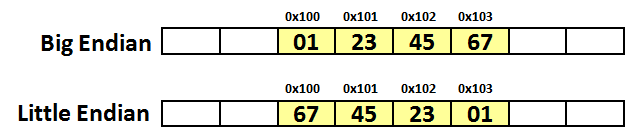
\includegraphics[width=1.0\linewidth]{images/lb_endian.png}
\end{center}
\end{frame}


\section{Аргументы функции main()}

\begin{frame}[fragile]
\frametitle{Аргументы функции main()} 
\begin{center}
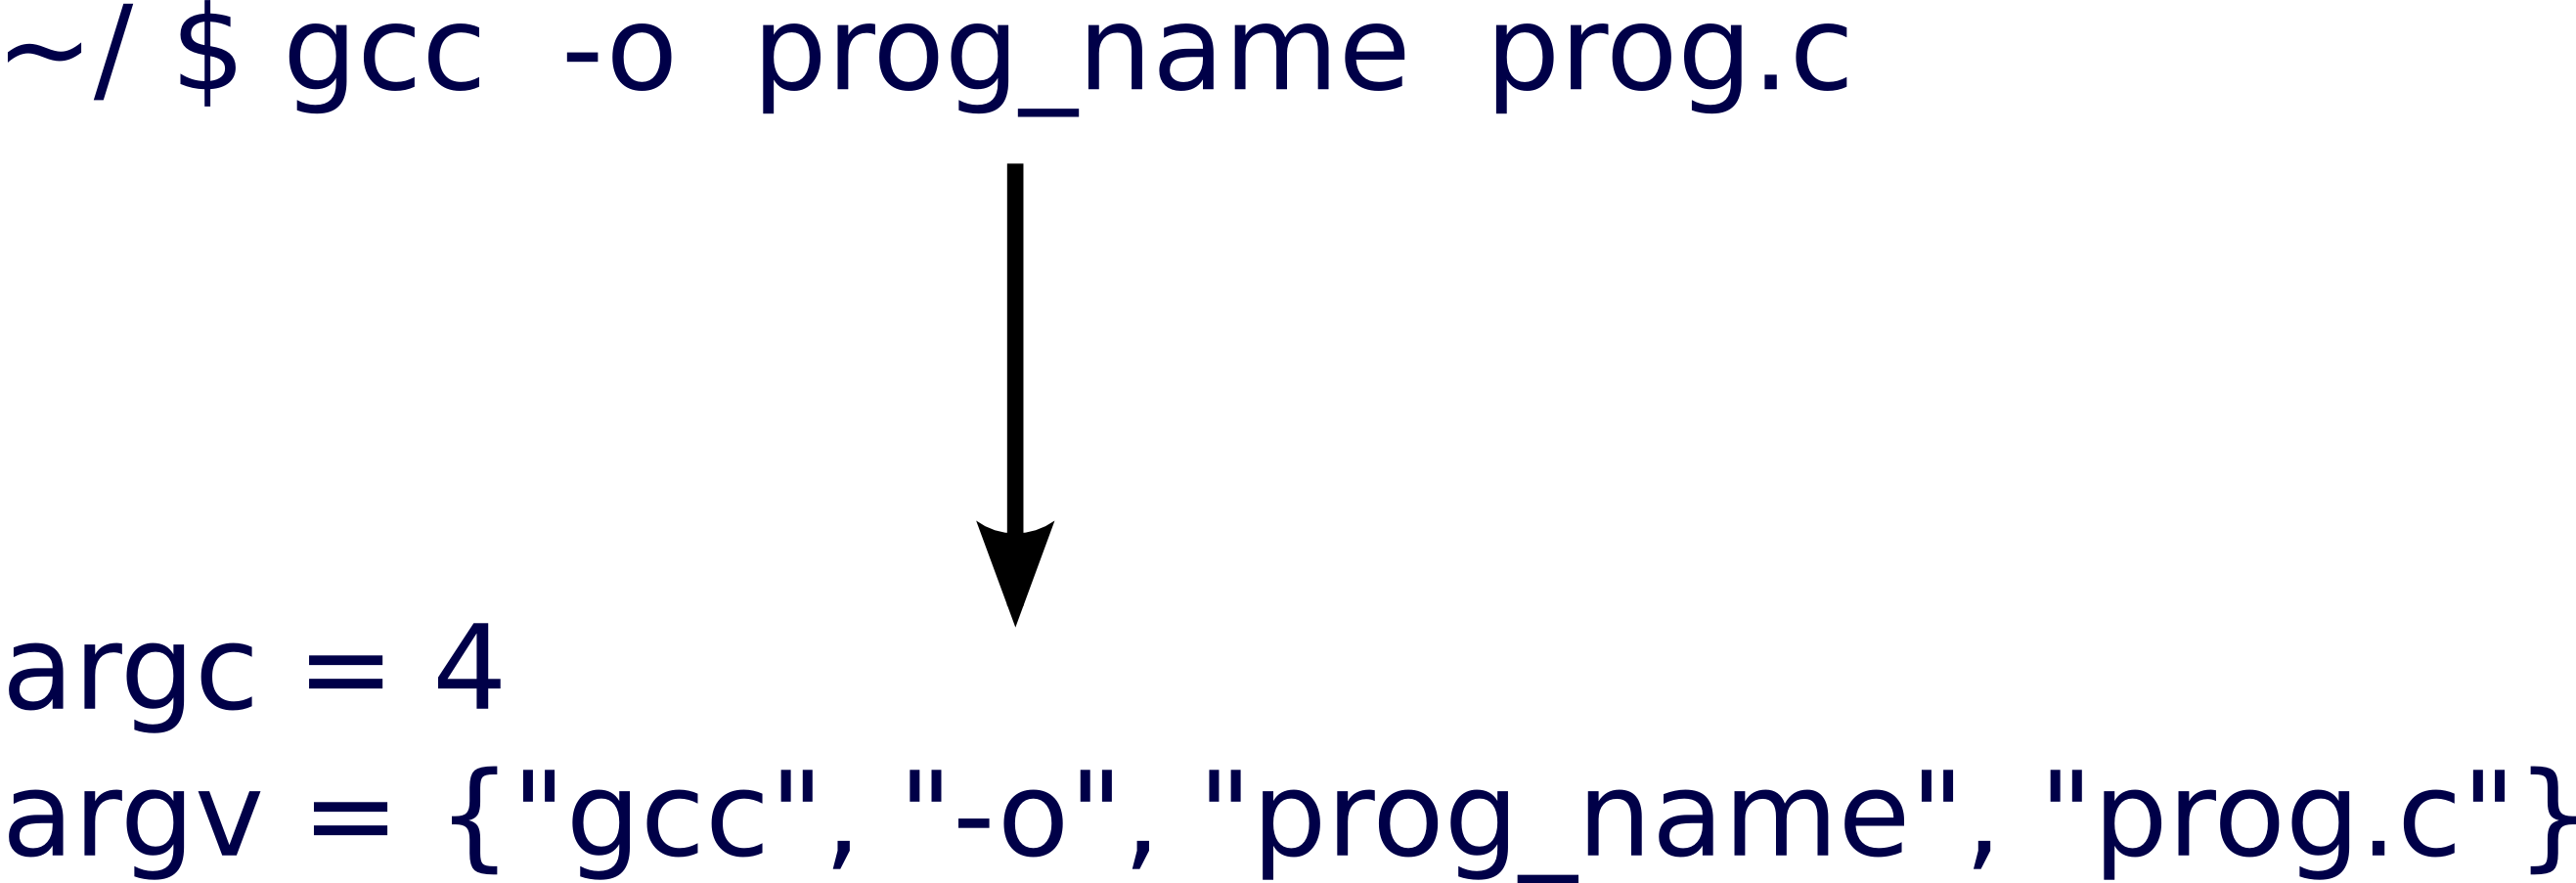
\includegraphics[width=1.0\linewidth]{images/function_argcargv.png}
\end{center}
\end{frame}

\begin{frame}[fragile]
\frametitle{Аргументы функции main()}  
\begin{center}
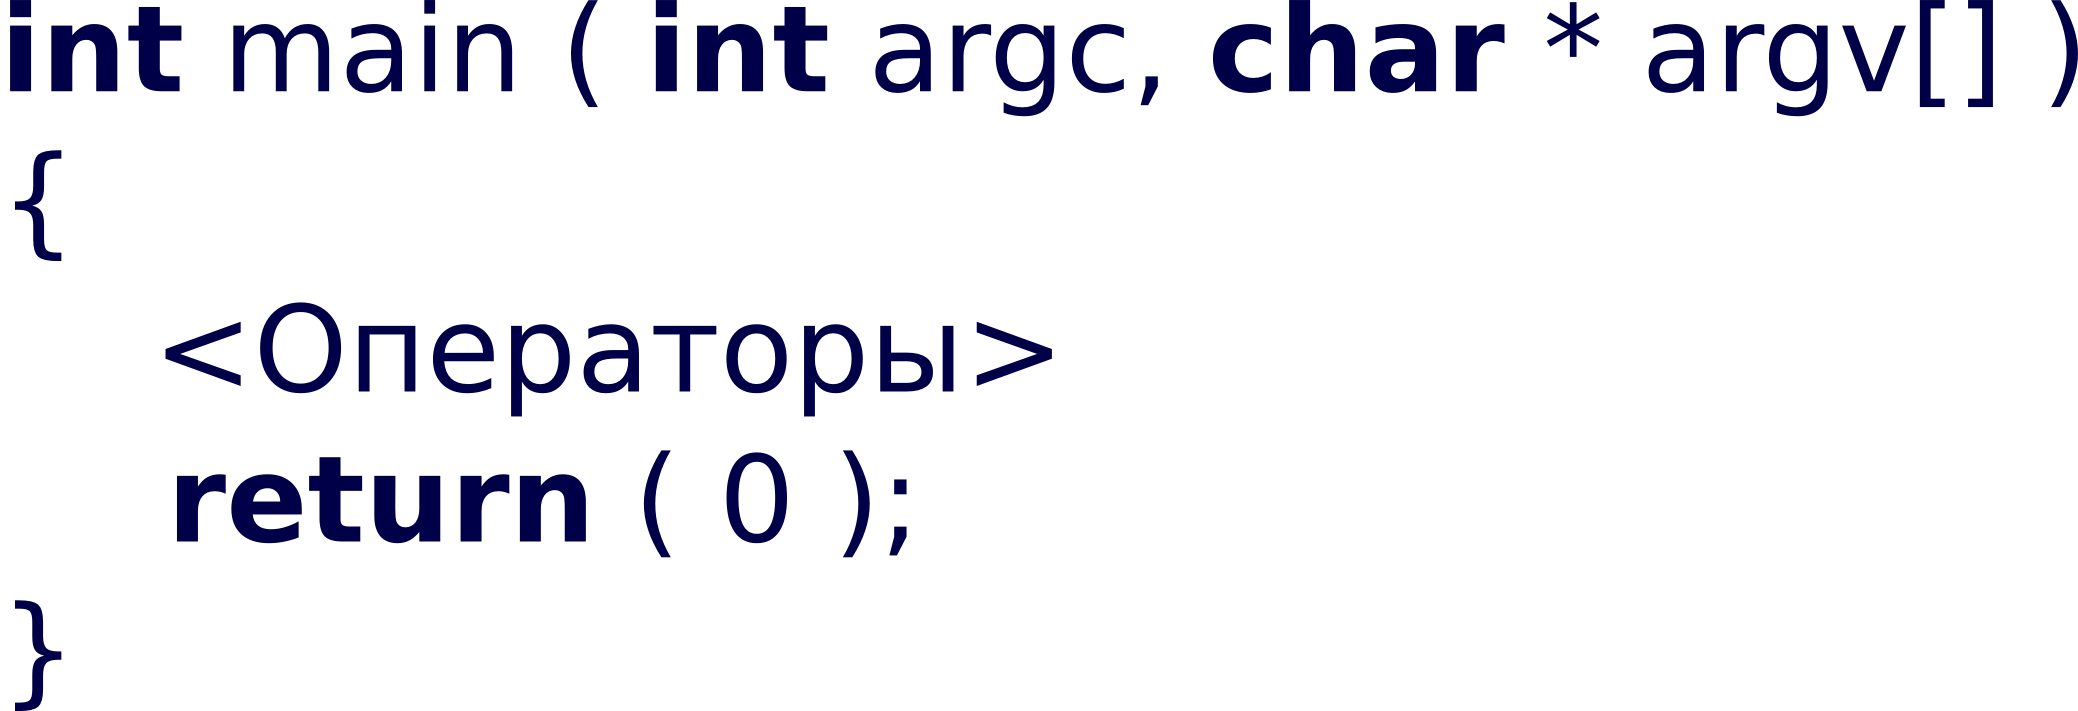
\includegraphics[width=0.7\linewidth]{images/function_syntax_main_args.png}
\end{center}
\begin{itemize}
\item argv -- параметры, передаваемые в функцию main
\item argc -- количество этих параметров
\end{itemize}
\end{frame}

\section{Сортировки за $O(n)$}


\begin{frame}[fragile]
\frametitle{Аргументы функции main()} 
\begin{itemize}
\item Сортировка подсчётом (count sort)
\item Цифровая сортировка (radix sort)
\end{itemize}
\end{frame}


\section{Задание}

\begin{frame}[fragile]
\frametitle{Задание} 
\begin{itemize}
\item Посчитать число строк, слов, символов в файле.
\item Написать аналог программы wc.
\item Контест Fail not found (задачи arguments, D и cp*)
\end{itemize}
\end{frame}

\end{document}
